% modified in response to reviewer comments
% formatted for IOP
\documentclass[12pt]{iopart}

\pdfminorversion=4

\usepackage{float}
\usepackage{units}
\usepackage{graphicx}
\usepackage{hyperref}

\newcommand{\be}{\begin{equation}}
\newcommand{\ee}{\end{equation}}
\newcommand{\bea}{\begin{eqnarray}}
\newcommand{\eea}{\end{eqnarray}}

\begin{document}

\title[Don't throw that video away! Reference Frames can fix Video Analysis with a Moving Camera]{Don't throw that video away! Reference Frames can fix Video Analysis with a Moving Camera}
\author{N T Moore}
\footnote{Present address:
Department of Physics, Winona State University, Winona, MN 55987, USA}
\ead{nmoore@winona.edu}

\date{\today}

\begin{abstract}
One common source of error in video analysis is camera movement.  The paper describes a simple frame of reference correction that students can employ to salvage otherwise corrupted video analysis data.  Two examples are provided. 
\end{abstract}

\noindent{\it Keywords\/}: video analysis, LoggerPro, frames of reference, kinematics

\submitto{\PED}

\maketitle

\section{Introduction} 
Video analysis is a convenient and fun way to collect kinematic position-time information for a motion that may not be otherwise accessible in the introductory lab.  The general procedure is to track the successive motion of an object via it's x and y pixel position over multiple frames of a video.  The technique has been around since at least 1894 \cite{nature_cat}!
  

One curriculum that uses video analysis as a learning support to construct and test ideas is Eugenia Etkina's ISLE approach to learning physics \cite{ISLE_overview}. 
For example, in the 2-D Projectile motion unit, one video \cite{ISLE_ball_video_source}, involves Dr. Etkina tossing a ball vertically while rolling across the room on rollerblades. If you are reading the paper on a computer, you might watch the video now \url{http://islevideos.net/experiment.php?topicid=2&exptid=95}.   

\begin{figure}[h]
\centering
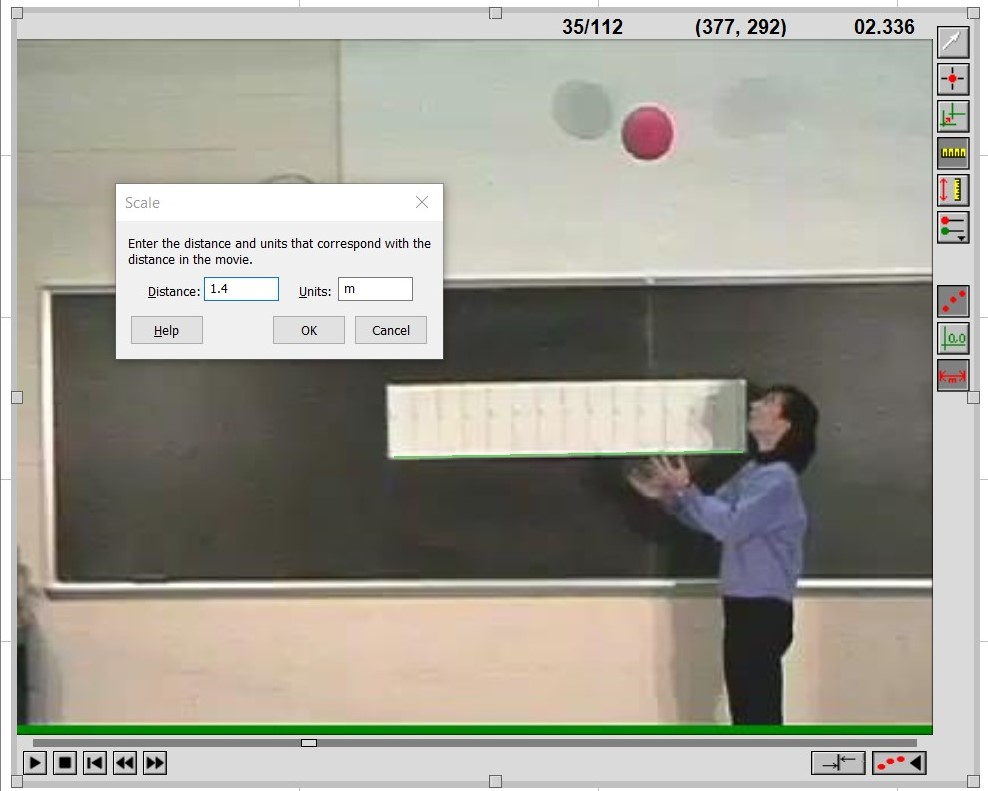
\includegraphics[width=\columnwidth]{figure_1_Etkina-calibration.jpg}
\caption{ 
A screenshot from the ISLE-based video website (developed by E. Etkina and D.T.Brookes).
The video has been imported for analysis in Vernier's LoggerPro software.    
Horizontal  scale is given via the set of vertical lines drawn on the chalkboard with assumed spacing of $10$cm. 
The (green) calibration stick is assumed to be 1.4m in length via lines drawn on the chalkboard.  The video can be downloaded from \cite{ISLE_ball_video_source} .
}
\label{Etkina-calibration}
\end{figure}

\begin{figure}[h]
\centering
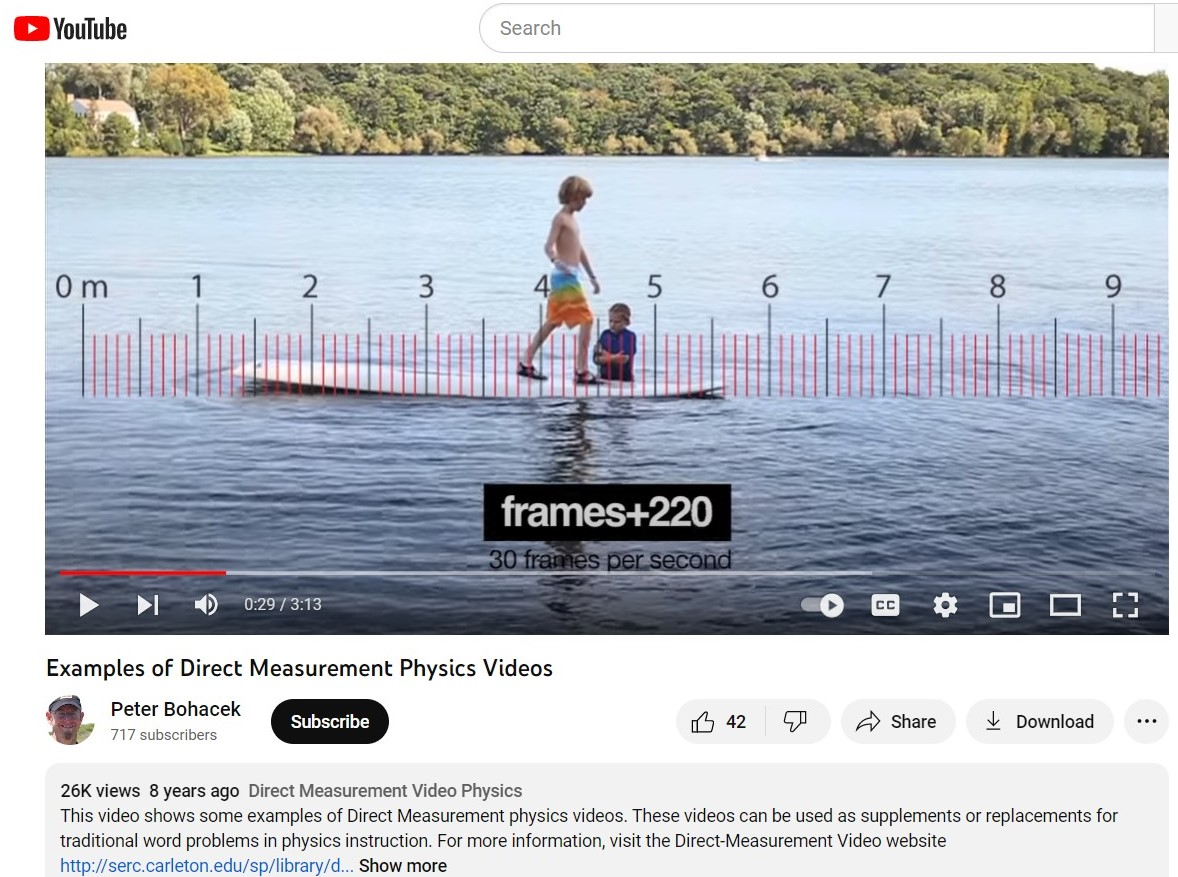
\includegraphics[width=\columnwidth]{figure_2_Bohacek-1.jpg}
\caption{A screenshot from Peter Bohacek's Direct Measurement Videos, \cite{Bohacek_youtube_intro}. In this case, position information is given by a drawn overlay added to the video via post-processing.
}
\label{Bohacek-1}
\end{figure}

Another set of teaching videos is Peter Bohacek's Direct Measurement Physics Videos, \cite{Bohacek_overview} .
These videos usually show physics in a ``real" setting (outside the classroom) and are again powerful and engaging tools.  

In both of these examples, students are presented with videos that can be analyzed frame by frame at constant time intervals.  Horizontal and vertical positions are available by either marks on a chalkboard (Etkina) or a computer drawn overlay (Bohacek).  

There are a number of video analysis software programs that allow students to analyze any old video they find or record with their cellphones.  ``Tracker'', \cite{Tracker}, is a free tool that works on a variety of platforms. Vernier's Logger Pro, \cite{LoggerPro}, often used for data acquisition, also contains video analysis software.  

In both of these packages, students repeatedly click on an object of interest and the software then collects time and 2D position data  in spreadsheet form.  However, the data collected is in units of an x,y pixel pair.  Conversion from pixel to physical dimension is a student task, and the quality of student results can depend on the ``calibration stick''\cite{calibration_stick} they employ.

\section{Fixing moving camera motion} 
Figures \ref{Etkina-calibration} and \ref{Etkina-dots-2} show the analysis process for the video in which Dr. Etkina throws a ball vertically while rollerblading across the classroom.  The video of this event was taken by a camera that followed Etkina, so via direct tracking of the ball, the horizontal component is lost.

However, if a student also tracks the motion of a seemingly immobile object, for example the center seam of the chalkboard, the center of the clock, a corner of the calibration sheets, etc, the student can recover the horizontal motion of the ball via vector subtraction.  Specifically, if you write  the ball's position relative to the classroom wall as, $X_{ball~wrt~wall}$, you can then express this position as a difference.
\bea
X_{ball~wrt~wall} &=& X_{ball~wrt~camera}-X_{clock~wrt~camera} \nonumber\\ 
Y_{ball~wrt~wall} &=& Y_{ball~wrt~camera}-Y_{clock~wrt~camera}\nonumber
\eea
This subtraction can be accomplished in LoggerPro as a ``calculated column'' or the data can be exported to a spreadsheet and the operation performed there.  

Results from this change of reference frame, using Logger Pro, are shown in figures \ref{Etkina-Y-T-plot} and \ref{Etkina-X-T-plot} . 
In the introductory curriculum, frames of reference sometimes seem dry or contrived, but in video analysis projects with a moving camera, thinking about the movement of a seemingly immobile reference frame can be a magic bullet.  Some video analysis programs, for example, Tracker, allow automatic tracking of motion within a moving frame of reference\cite{tracker_planets}.  

\begin{figure}[h]
\centering
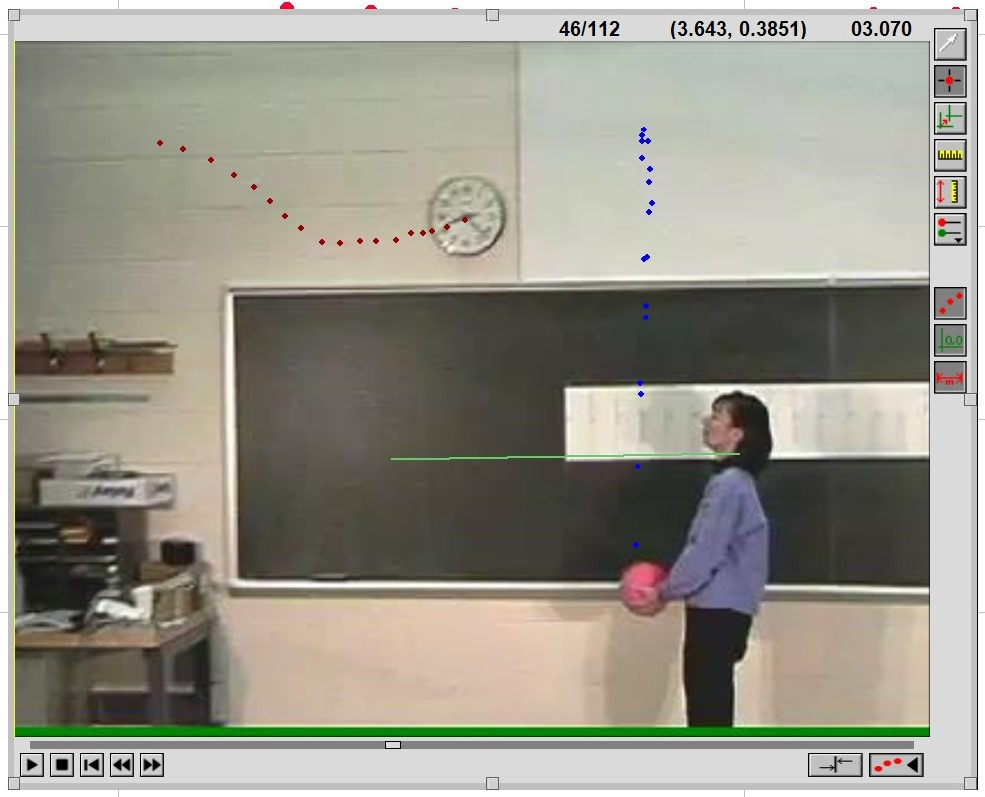
\includegraphics[width=\columnwidth]{figure_3_Etkina-dots-2.jpg}
\caption{
A screenshot from LoggerPro, showing both the track of the pink ball (blue dots) and the track made by the clock (red dots).  Note, the clock is attached to a concrete block wall, so the red dots also show the motion of the camera.  
While the ball is certainly moving across the classroom horizontally, the moving camera does not show this motion in the track of blue dots.
The position of the ball \textit{with respect to the classroom} can be generated via vector subtraction of the ball-camera and clock-camera reference frames.
}
\label{Etkina-dots-2}
\end{figure}

\begin{figure}[h]
\centering
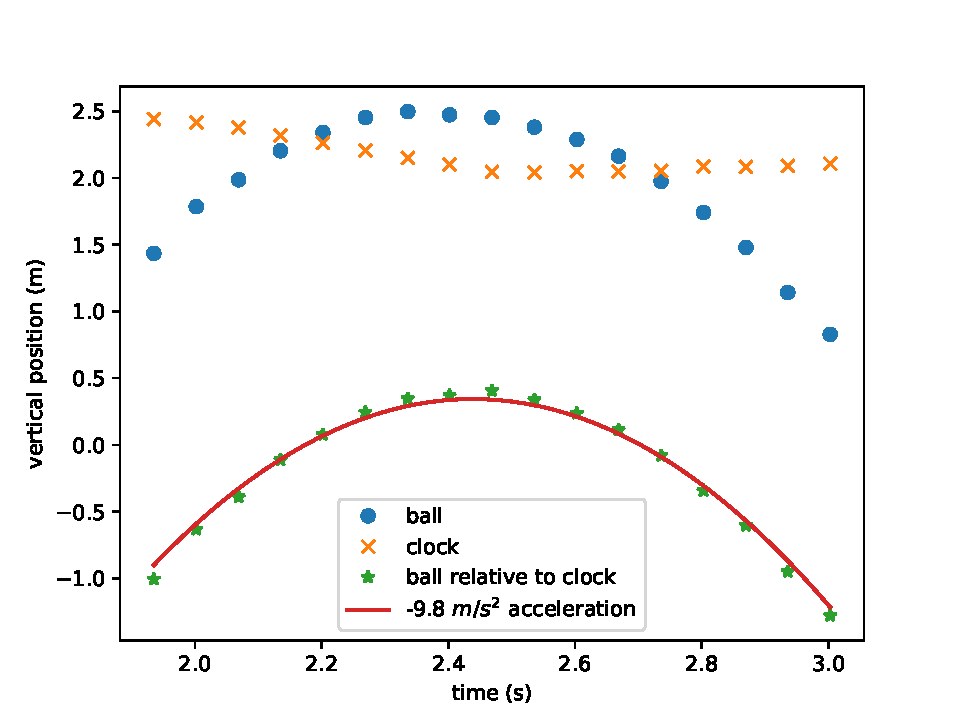
\includegraphics[width=\columnwidth]{figure_4_Etkina-Y-T-plot.pdf}
\caption{
A plot showing the vertical position of the clock, the ball, and the difference between the two, the vertical position of the ball relative to the clock. 
Looking carefully, you can see that correcting for the relative motion of the camera eliminates the asymmetry in the direct measurement of the ball's altitude.  
}
\label{Etkina-Y-T-plot}
\end{figure}

\begin{figure}[h]
\centering
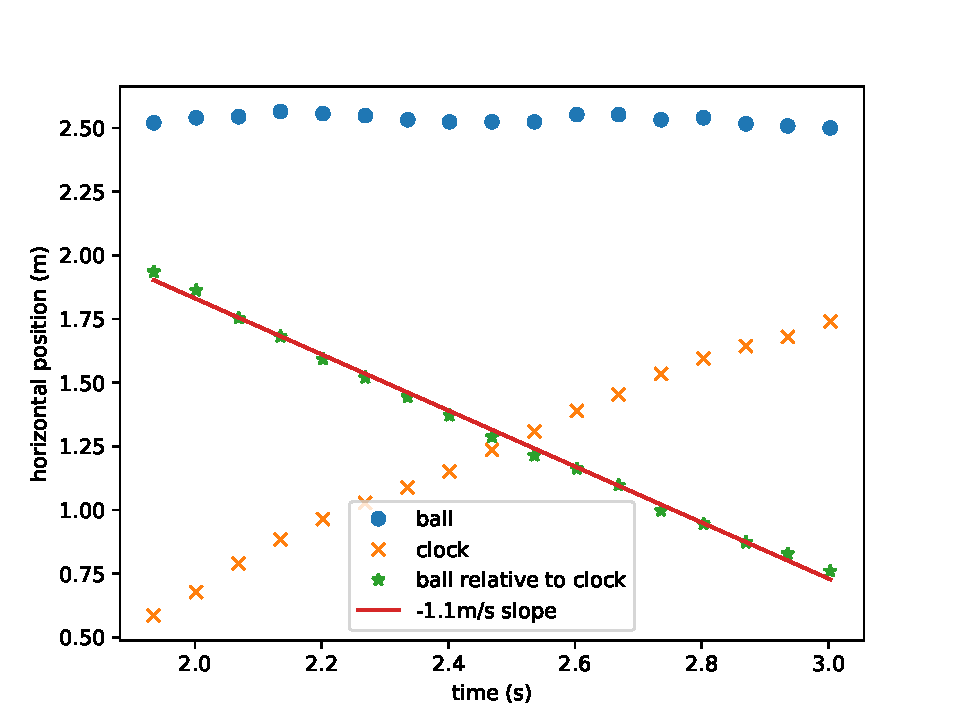
\includegraphics[width=\columnwidth]{figure_5_Etkina-X-T-plot.pdf}
\caption{
A plot from LoggerPro showing the horizontal position of the clock, the ball, and the difference between the two, ie the horizontal position of the ball relative to the clock.  This graph shows how motion hidden by a moving camera can be recovered if you subtract away the (camera) motion of a fixed reference.
}
\label{Etkina-X-T-plot}
\end{figure}

% added to get the figures to line up with sections of the text
\clearpage

\section{Example: a bear falls out of a tree}
To further illustrate how useful this approach can be, consider this 2003 video of a bear being removed from a tree in Missoula Montana via a tranquilizer gun and a trampoline. \url{https://www.youtube.com/watch?v=9KiJnTGoPPI} \cite{bear_video_source}.  
There are quite a few different application topics available in the video, and some of my students are outraged that the bear was so made fun of by the Missoula fire, wildlife, and police departments.  

So, an ethical question: ``Assuming the bear had to be removed from the tree, was bouncing it off a trampoline a humane thing to do?''  With encouragement, the students can develop this question into a quantifiable measure, eg, ``What would the bear's speed be if there was no trampoline in place?''  There are many graphs online that show the fatality risk for pedestrians who are struck by cars at different speeds, for example \cite{AccidentRisk}, and it seems realistic to extrapolate this to a decrease in harm to the bear if its final velocity is reduced.

\begin{figure}[h]
\centering
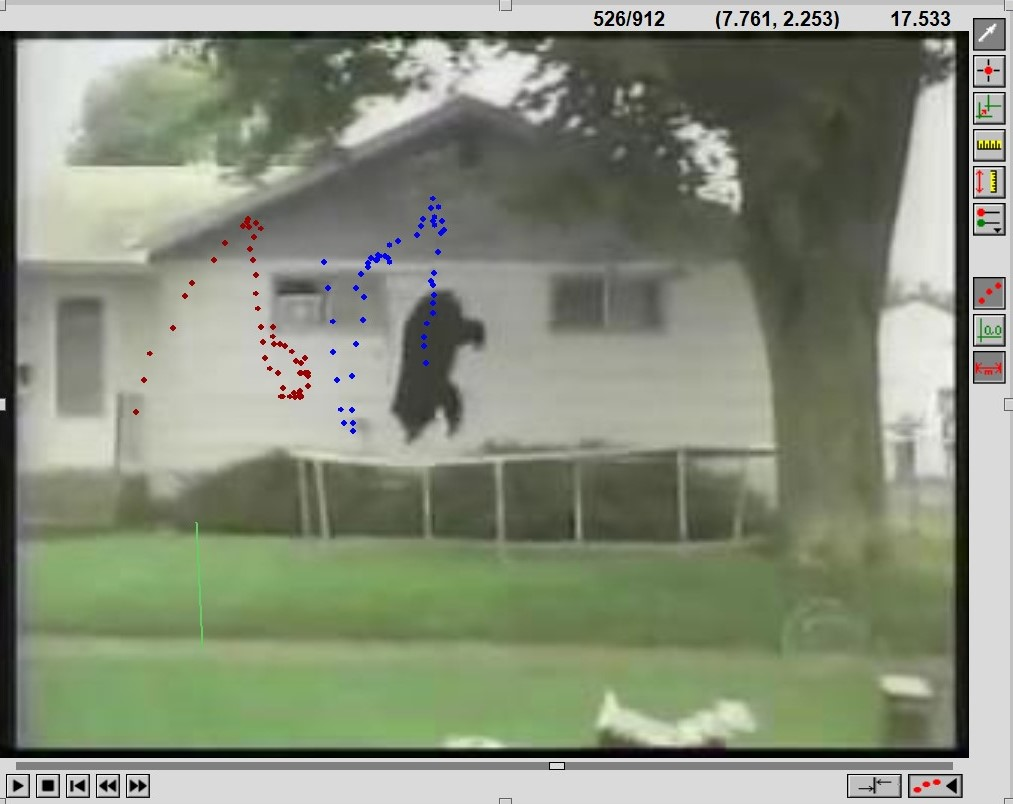
\includegraphics[width=\columnwidth]{figure_6_bear-dots.jpg}
\caption{
A screenshot from LoggerPro, showing the position-time track for both the bear and the lower left corner of the house's left transom window. The calibration used is the trampoline's leg height of $1$m.  The calibration stick has drifted off to the left because of the movement of the camera.  The calibration length is only an estimate and should probably be back fit to the appropriate gravitational acceleration value for the bear's free-fall.
}
\label{bear-dots}
\end{figure}

The bear video was shot by a professional videographer, Mark Hoyoak, and the focus of the camera follows the bear.  Ignoring the early parts of the bear's fall when the zoom level changes, the video provides a falling body, tracked by a moving camera.  If you consider one of the house's transom windows to be a static reference, camera movement can be removed.

\begin{figure}[ht]
\centering
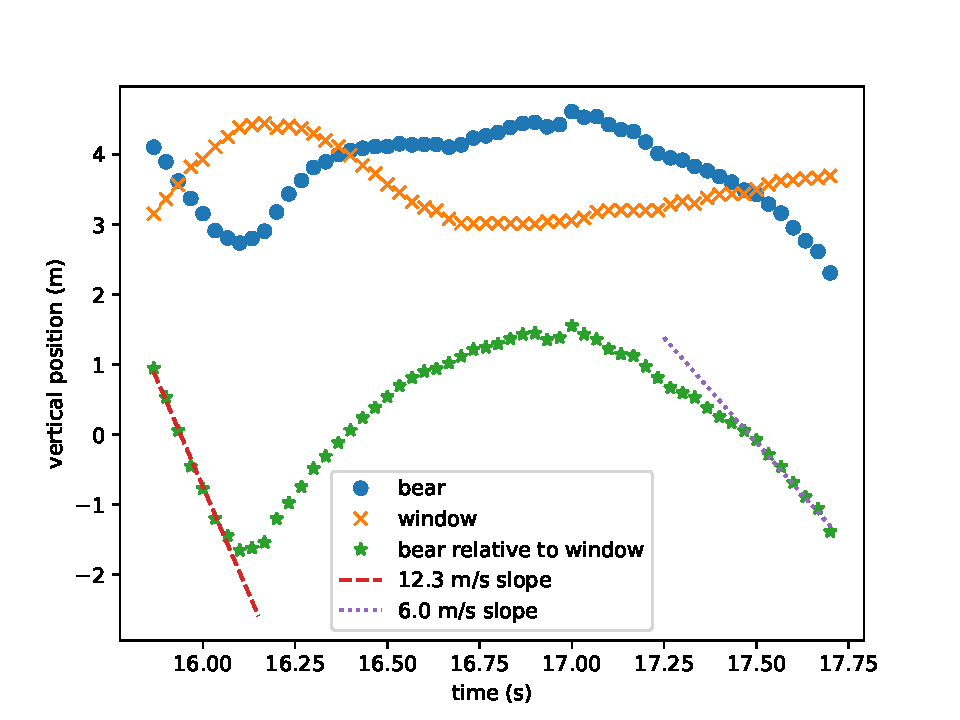
\includegraphics[width=\columnwidth]{figure_7_bear-speed.pdf}
\caption{
A plot showing the vertical position-time graph for both the bear, the lower left corner of the house's left transom window and the bear's (calculated)  motion relative to the window. 
}
\label{bear-speed}
\end{figure}

This analysis is shown in figures \ref{bear-dots}, \ref{bear-speed}, and \ref{bear-quadratic}.
The analysis assumes a trampoline leg height of $1$ meter, which, based on the extracted gravitational acceleration values, is probably inaccurate.
 
 Straight-line fits to the bear's vertical position give speeds of $12.3m/s\approx27mph\approx44kmph$ as the bear hits the trampoline, and $5.9m/s\approx13mph\approx21kmph$ at about the same altitute after bouncing off the trampoline.  Based on the data in Figure 1b of \cite{AccidentRisk} this corresponds to a reduction of pedestrian fatality risk from $5\%$ to less than $1\%$.  Extrapolating from vehicle fatality data, one could arge that in addition to being good comedy, using a trampoline in this case is humane wildlife management.     
 
 In addition to applications in mechanics, it is likely that this moving frame of reference technique could be applied in the introductory astronomy curriculum, for example \cite{tracker_planets} or \cite{retrograde_planets}.
     
\begin{figure}[h]
\centering
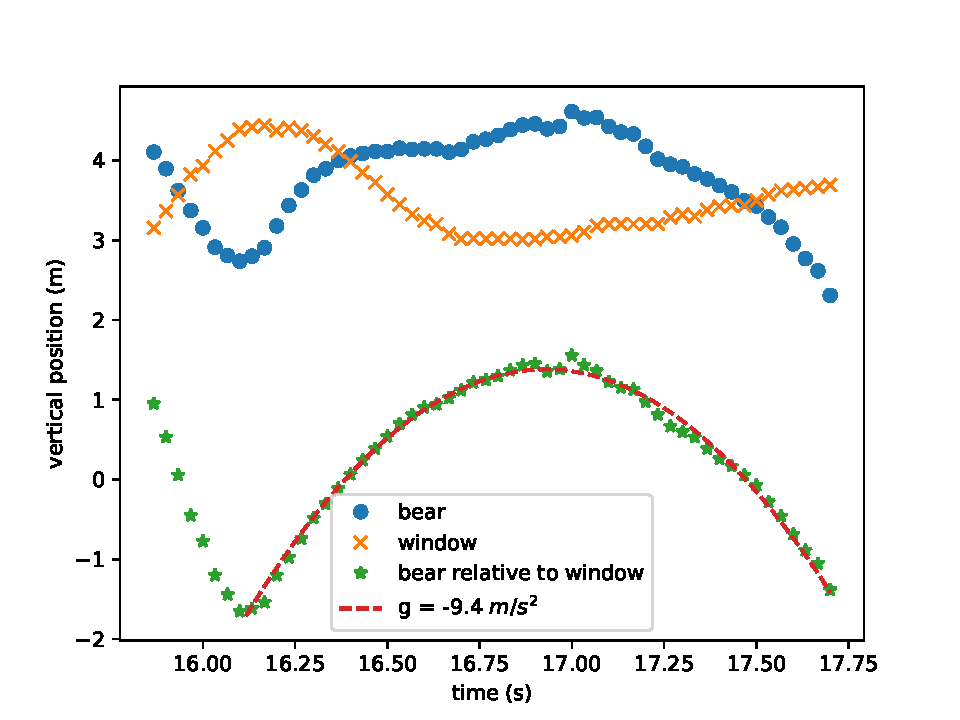
\includegraphics[width=\columnwidth]{figure_8_bear-quadratic.pdf}
\caption{
A quadratic fit to the bear's position (relative to the window) shows a $time^2$ polynomial with gravitational acceleration of about $g=9.4\pm 0.1~m/s^2$.  This is obviously not the standard $g$ value from the textbook and suggests both ``clicking error'' in tracking the motion and calibration error in assuming the trampoline is $1$ meter high. The real height of the trampoline could be backwards fit by scaling the observed $g$ value to $9.8$ as described in \cite{backwards_fit}. 
Never-the-less, the corrected motion (unlike that of the bear from the moving camera) is clearly quadratic, which is a demonstration of the utility of the approach used in this paper.
}
\label{bear-quadratic}
\end{figure}

\section{Conclusion}
Cellphone video is everywhere in a way that was unimaginable 20 years ago.  Most of the videos that students might take for a kinematics assignment won't be shot from a tripod with a constant depth of field.  Accordingly, talking about how to use topics from Physics to correct ``errors'' in video data collection can be empowering for students.  If there's a fixed reference, a student no longer needs to be told, ``That video is bad, go take it again...''.

%\begin{acknowledgments}
\ack
The work would not have been possible without Mark Hoyoak's excellent videography.  Thanks also to Eugenia Etkina for introducing me to video analysis many years ago.  Thanks also to Peter Bohacek for his inspiring talks and amazing Direct Motion Video examples.  

%\end{acknowledgments}

\section*{References}
\begin{thebibliography}{99}

\bibitem{nature_cat}
Marey M
1894
Photographs of a Tumbling Cat. 
{\it Nature }
{\bf 51} 
80
%https://doi.org/10.1038/051080a0

\bibitem{ISLE_overview}  
The ISLE approach to learning physics is described in 
Etkina E 
2015
Millikan award lecture: Students of physics—Listeners, observers, or collaborative participants in physics scientific practices?
{\it American Journal of Physics}
{\bf 83(8)}
669
%669-679
%DOI: 10.1119/1.4923432 
and 
Brookes D T and Etkina E
2010
Physical Phenomena in real time
{\it Science}
{\bf 330}
605
%605-606
Here is a pointer to the video archive I'm using \url{http://islevideos.net/} .
  
\bibitem{ISLE_ball_video_source}
The ball toss video used in the first part of the paper is available for download at \url{http://islevideos.net/experiment.php?topicid=2&exptid=95} .

\bibitem{Bohacek_youtube_intro}
See the excellent introduction at 
\url{https://www.youtube.com/watch?v=QsGMKv8Lrew}. This screenshot comes from \url{https://www.youtube.com/watch?v=CMpc1cXqC7s}.

\bibitem{Bohacek_overview} Peter Bohacek's YouTube channel contains a large number of these videos \url{https://www.youtube.com/user/bohacekphysics}.  
A nice overview of the approach he takes is given in \url{https://www.youtube.com/watch?v=QsGMKv8Lrew}. 
These videos are available as a commercial curriculum at \url{https://www.pivotinteractives.com/} .

\bibitem{Tracker} Tracker is a free, open-source tool that you can install on your computer or run in a web browser.  It is available online at \url{https://physlets.org/tracker/} .

\bibitem{LoggerPro} Vernier's LoggerPro is typically used for lab data acquisition but it contains an excellent video analysis tool that this paper employs. 
\url{https://www.vernier.com/product/logger-pro-3/}

\bibitem{calibration_stick} Here is the help page for calibration sticks in Tracker \url{https://physlets.org/tracker/help/frameset.html}.  The process in LoggerPro is similar.

\bibitem{tracker_planets}
Balaton M, Cavadas J, Simeão Carvalho P, and Lima J
2021
Programming Ozobots for teaching astronomy
{\it Physics Education}
\textbf{56(4)}
045018
%Citation Mariana Balaton et al 2021 Phys. Educ. 56 045018
%DOI 10.1088/1361-6552/abfb44

\bibitem{bear_video_source}
There are many copies of this video on the web.  It seems that the original video was taken by Mark Hoyoak of KPAX News in Montana on September 9, 2003.  The clip was subsequently featured on national news and comedy programs.  For an overview, see \url{https://www.youtube.com/watch?v=jB47Vucoj2o} .
   
\bibitem{AccidentRisk} 
%https://doi.org/10.1016/j.aap.2009.02.002
Rosén E and Sander U
2009
Pedestrian fatality risk as a function of car impact speed
{\it Accident Analysis and Prevention}
\textbf{41(3)} 
536
%536-542

\bibitem{backwards_fit}
Rodrigues M and Simeão Carvalho P 
2013
Teaching physics with Angry Birds: exploring the kinematics and dynamics of the game
%© 2013 IOP Publishing Ltd
{\it Physics Education}
\textbf{48(4)}
431
%Citation M Rodrigues and P Simeão Carvalho 2013 Phys. Educ. 48 431
%DOI 10.1088/0031-9120/48/4/431

\bibitem{retrograde_planets}
Guerra A and Simeão Carvalho P
2016
Orbital motions of astronomical bodies and their centre of mass from different reference frames: a conceptual step between the geocentric and heliocentric models
{\it Physics Education}
\textbf{51(5)}
055012
%Citation André G C Guerra and Paulo Simeão Carvalho 2016 Phys. Educ. 51 055012
%DOI 10.1088/0031-9120/51/5/055012

\end{thebibliography}

\end{document}
